\documentclass[t]{beamer}

%\documentclass[handout, t]{beamer}
\setbeamertemplate{navigation symbols}{}

 
\usepackage{amsfonts}
\usepackage{mathrsfs}
\usepackage{amsmath}
\usepackage{multicol}

\usepackage{bm}
\usepackage[UTF8]{ctex}
\usetheme{AnnArbor}
\usefonttheme{serif}
\useinnertheme{rounded}
%\usecolortheme{crane}
\setbeamertemplate{blocks}[rounded][shadow=true]

\usepackage{graphicx}

\setmainfont{Times New Roman}
\setCJKmainfont{Microsoft YaHei}
\usepackage{tikz}
\usetikzlibrary{arrows, decorations.pathmorphing, backgrounds, positioning, fit, petri, automata}
\tikzset{>=stealth}

\hypersetup{pdfpagemode=FullScreen}
\renewcommand{\Pr}{\mathbb{P}}
\newcommand{\E}{\mathbb{E}}

\usepackage{blkarray}


\setbeamercolor{block title}{bg=red!10!white}
\setbeamercolor{block body}{bg=gray!5!white}

\newcommand{\dif}{{\;\rm d}}

\usepackage{listings}


\lstset{
  language=Python, % 设置语言
  basicstyle=\ttfamily, % 设置字体族
  breaklines=true, % 自动换行
  keywordstyle=\bfseries\color{blue}, % 设置关键字
  ndkeywordstyle=\bfseries\color{blue}, % 设置关键字
  classoffset=0,
  emph=[0]{self, plt, pd, np, print, sm, sns, stats, plot_acf,plot_pacf, adfuller,acorr_ljungbox, True, False, None, diff, heatmap}, % 指定强调词,如果有多个,用逗号隔开
  emphstyle=\bfseries\color{magenta!90!black}, % 强调词样式设置
  classoffset=1,
  moreemph=[1]{plot, text, title, show, scatter, as, figure, xlabel, ylabel, fit, mean, var, skew, kurt, distplot,rcParams, std, isf, summary,predict,cov,corr, cumprod, mul, repeat}, % 设置更多的关键字,用逗号分隔
  emphstyle=\bfseries\color{blue}, % 强调词样式设置
  classoffset=0,
  commentstyle=\itshape\color{gray}, % 设置注释样式,斜体,浅灰色
  stringstyle=\bfseries\color{green!50!black}, % 设置字符串样式
  columns=flexible,
  numberstyle=\footnotesize, % 缩小行号
}

\begin{document}
\fontsize{11}{18}\selectfont


\CTEXindent


\title{第三章~~证券业数据分析}

\author{主讲:方杰、李烜}
\date{福建江夏学院金融学院}

\maketitle

\begin{frame}[fragile]{本章内容}
\begin{multicols*}{2}
    \tableofcontents
    
\end{multicols*}

\end{frame}


\section{收益率描述性统计分析}
\subsection{收益率的统计特征}


\begin{frame}[fragile]{收益率的统计特征}
\begin{enumerate}
    \item 期望收益(均值) :均值是统计中用于描述数据集中位置的统计量。
    是描述集中趋势统计特征中最具代表性的数值
    \item  风险(方差) :方差在统计学中是用于衡量一组
    数据离散程度的统计量,它描述
    了一组数据对其均值的偏离程度
    \item   峰度和偏度:偏度又称偏态或偏态系数,是用于衡量数据分布非对称性的数字特征;峰度是衡量数据
    离群度的指标,也是对概率分布形状的刻画
\end{enumerate}
\end{frame}




\begin{frame}[fragile]{期望收益(均值)}
    在Python的pandas库中,求均值的函数为\verb|mean|
\begin{lstlisting}
    df.mean(axis=0)
\end{lstlisting}

默认对各列求均值,\verb|axis=1|表示对各行求均值。
\begin{block}{举例:}
    \begin{lstlisting}
import pandas as pd 
#导入沪深300日收益率数据
csi300_returns = pd.read_excel('文件路径', index_col=0) 
csi300_means = csi300_returns.mean()     # 计算日收益率
print('日平均收益率:', csi300_means)
\end{lstlisting}
\end{block}
\end{frame}


\begin{frame}[fragile]{风险(方差)}
\begin{lstlisting}
    df.var(axis=0, skipna=True)
\end{lstlisting}
\begin{itemize}
    \item 默认对各列求方差,\verb|axis=1|表示对各行求方差
    \item \verb|skipna| 默认排除空值
\end{itemize}
\begin{block}{举例:}
    \begin{lstlisting}
import pandas as pd
# csi300_returns为沪深300日收益率数据
csi300_vars=csi300_returns.var() 
print( '收益率的方差:', csi300_vars)
\end{lstlisting}
\end{block}
\end{frame}



\begin{frame}[fragile]{偏度}
    偏度(Skewness)又称偏态或偏态系数,是用于衡量数据分布非对称性的数字特征
\[{\rm Skew}=\E\left[\left(\frac{r-\mu}{\sigma}\right)^3\right]=\frac{\E[(r-\mu)^3]}{\sigma^3} \]
\begin{lstlisting}
    df.skew(axis=0, skipna=True)
\end{lstlisting}
\begin{itemize}
    \item 偏度${\rm Skew}<0$:呈现左偏
    \item 偏度${\rm Skew}>0$:呈现右偏
    \item 偏度${\rm Skew}=0$:分布相对均匀
\end{itemize}
\end{frame}


\begin{frame}[fragile]{峰度}
峰度(Kurtosis)是衡量数据
离群度的指标,也是对概率分
布形状的刻画。
\[{\rm Kurt}=\E\left[\left(\frac{r-\mu}{\sigma}\right)^4\right]=\frac{\E[(r-\mu)^4]}{\sigma^4} \]

\begin{lstlisting}
    df.kurt(axis=0, skipna=True)
\end{lstlisting}

\begin{itemize}
    \item 峰度${\rm Kurt}=3$,此时是正态分布,也称为常峰态
    \item 峰度${\rm Kurt}>3$,尖峰态,相较于正态分布而言具有
    较高的峰部和更长的尾部
    \item 峰度${\rm Kurt}<3$,低峰态,相较于正态分布而言具有较
    平坦的峰部和更短更细的尾部
\end{itemize}
\end{frame}


\begin{frame}[fragile]{峰度和方差之间的关系}
峰度和方差之间的关系紧密,区别微妙。

峰度和方差的不同在于,方差衡量了随机变
量偏离均值的分布状况,而峰度衡量了随机变量大幅偏离均值的可能性。
\begin{itemize}
    \item 方差较大,意味着随机变量分布较为分散,并没有聚集在均值附近。
    \item 在给定方差情况下,峰度值
较大意味着方差贡献主要是来自少数的极值,而不是
偏离程度较为温和的数值。
\end{itemize}
\end{frame}


\subsection{收益率的分布特征}

\begin{frame}[fragile]{正态分布}
\begin{center}
    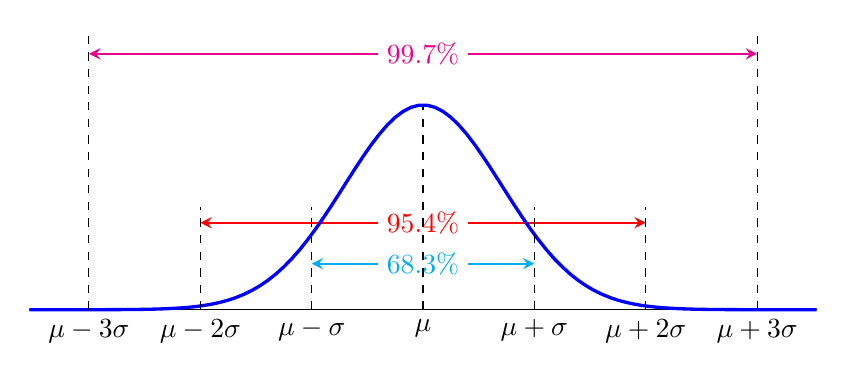
\begin{tikzpicture}[yscale=1.3]
\draw[<->, thick, color=cyan](1.414,.45)--node[fill=white]{68.3\%}(-1.414,.45);
\draw[<->, thick, color=red](1.414*2,.85)--node[fill=white]{95.4\%}(-1.414*2,.85);
\draw[<->, thick, color=magenta](1.414*3,2.5)--node[fill=white]{99.7\%}(-1.414*3,2.5);
\draw[dashed](0,0)node[below]{$\mu$}--(0,2);
\draw(-5,0)--(5,0);
\draw[domain=-5:5, samples=100, very thick, color=blue] plot(\x, {2*exp(-.5*\x*\x)});

\draw[dashed](1.414,0)node[below]{$\mu+\sigma$}--(1.414,1);
\draw[dashed](2.828,0)node[below]{$\mu+2\sigma$}--(2.828,1);
\draw[dashed](-1.414,0)node[below]{$\mu-\sigma$}--(-1.414,1);
\draw[dashed](-2.828,0)node[below]{$\mu-2\sigma$}--(-2.828,1);
\draw[dashed](4.243,0)node[below]{$\mu+3\sigma$}--(4.243,2.75);
\draw[dashed](-4.243,0)node[below]{$\mu-3\sigma$}--(-4.243,2.75);

    \end{tikzpicture}
\end{center}

正态分布的累积分布函数(Cumulative Distribution Function, CDF)的公式如下:
\[F(x)=\frac{1}{\sqrt{2\pi}\sigma}\int^x_{-\infty}\exp\left[-\frac{(t-\mu)^2}{2\sigma^2}\right]{\rm d} t \]

%概率密度函数(Probability Density Function, PDF)的公式如下:
% \[f(x)=\frac{1}{\sqrt{2\pi}\sigma}\exp\left[-\frac{(x-\mu)^2}{2\sigma^2}\right] \]
% 对应的
\end{frame}



\begin{frame}[fragile]{正态分布(cont.)}
当均值$\mu=0$,方差$\sigma=1$时,正态分布称为标准正态分布
\[X\sim \mathcal{N}(\mu,\sigma^2),\qquad Z=\frac{X-\mu}{\sigma}\sim  \mathcal{N}(0,1)\]

正态分布具有很多良好的特性,许多概率分布可以用它来近似,因此多数情况下对变量进行研究的时候,往往先假设该变量的概率分布为正态分布

\end{frame}

\begin{frame}[fragile]{正态分布的直观观测}
要得知一组数据是否符合正态分布,简单的方法是绘制直方图(histogram)来直观地观测。

\begin{lstlisting}
    import seaborn as sns
    sns.distplot(a, hist=True, kde=True, label=None)
\end{lstlisting}
\begin{itemize}
    \item \verb|seaborn| 是基于 Python 且非常受欢迎的图形可视化库
    \item \verb|a| 是待分析的一维数组变量
    \item \verb|hist| 默认显示为条形图
    \item \verb|kde| 默认直方图高度显示为密度而非计数
    \item \verb|label| 控制图像中的图例标签显示内容,只能显示英文形式
\end{itemize}
\end{frame}



\begin{frame}[fragile]{举例:沪深300指数的日收益率数据直方图绘制}
\begin{lstlisting}
import seaborn as sns
import matplotlib.pyplot as plt
plt.rcParams['axes.unicode_minus'] = False
# 解决负号无法正常显示的问题
sns.set(font='SimHei', style='white')
# 解决中文无法正常显示的问题,这里使用黑体字
sns.distplot(csi300_returns)
plt.xlabel('收益率')
plt.ylabel('概率密度')
plt.show()
\end{lstlisting}
\end{frame}

\begin{frame}[fragile]{正态分布的统计检验:K-S检验}
Kolmogorov-Smirnov检验(K-S检验),可用于检验一个分布与理想分布是否相同。
\begin{itemize}
    \item $H_0$: 样本数据的分布与理想分布无显著差异
    \item $p$-value: 原假设为真时样本观察结果出现的概率
\begin{itemize}
    \item $p$-value$>5\%$,$H_0$成立;
    \item $p$-value$<5\%$,$H_0$不成立
\end{itemize}
\end{itemize}

\begin{lstlisting}
    from scipy.stats import kstest
    kstest(rvs, cdf, args)
\end{lstlisting}



\end{frame}

\begin{frame}[fragile]{K-S检验(cont.)}
\begin{lstlisting}
    kstest(rvs, cdf, args)
\end{lstlisting}
\begin{itemize}
    \item \verb|rvs| 指定要统计的数据(随机变量样本)。
    \item \verb|cdf| 指定利用哪个概率分布对数据/变量进行分布拟合优度检验。
    \begin{itemize}
        \item 当\verb|cdf='norm'|时,要检验的是正态分布;
        \item 当\verb|cdf='chi2'|时,检验卡方$\chi^2$分布;
        \item 当\verb|cdf='t'|时,检验$t$分布;
        \item 当\verb|cdf='f'|时,检验$F$分布
    \end{itemize}
    
    \item \verb|args| 输入当\verb|rvs|或\verb|cdf|是字符串或引用对象时使用,输入形式为元组、序列。    
    当
    \verb|cdf='norm'|时,\verb|args=(rvs.mean(),rvs.std())|, 即待检验数据的均值和方差
    \item 该函数会返回两个值,一个是K-S检验统计量,另一个是$p$-value值
\end{itemize}
\end{frame}


\begin{frame}[fragile]{正态分布的K-S检验}
沪深300指数的日收益率数据(\verb|csi300_returns|)进行K-S检验
\begin{lstlisting}
from scipy.stats import kstest 
ks_results = kstest(csi300_returns['收益率'], 'norm', 
             (csi300_returns.mean(), csi300_returns.std()))
print(ks_results)
\end{lstlisting}
\end{frame}

\begin{frame}[fragile]{补充:检验正态分布的Jarque-Bera检验}
沪深300指数的日收益率数据(\verb|csi300_returns|)进行Jarque-Bera检验
\begin{lstlisting}
from scipy.stats import jarque_bera
jb_results = jarque_bera(csi300_returns['收益率'])
print(jb_results)
\end{lstlisting}
\end{frame}



\begin{frame}[fragile]{$t$分布}
\[t=\frac{X}{\sqrt{Y/n}}\sim t(n)\]
其中:$X\sim \mathcal{N}(0,1),\qquad Y\sim \chi^2(n)$

$t$分布与正态分布主要区别在于,$t$分布用小样本来估计呈正态分布且方差未知的分布
\end{frame}


\begin{frame}[fragile]{$t$分布的检验步骤}
\begin{enumerate}
    \item 对样本数据进行$t$分布拟合
    \begin{lstlisting}
        stats.t.fit(样本数据)
    \end{lstlisting}
    \item 基于分布拟合的结果,进行K-S检验
    \begin{lstlisting}
        kstest(rvs, 't', (df, loc, scale))
    \end{lstlisting}
\end{enumerate}
\end{frame}


\begin{frame}[fragile]{$t$分布的检验}
\begin{lstlisting}
from scipy import stats
#对收益率进行t分布拟合
args = stats.t.fit(csi300_returns['收益率']) 
# 拟合后获取的args值分别为自由度(df)、
# 位置参数(loc)、尺度参数(scale)
print(args) 
# 对收益率数据进行t分布的KS统计检验
ks_results = kstest(csi300_returns['收益率'], 't', 
                        (args[0], args[1], args[2]))
print(ks_results)
\end{lstlisting}
\end{frame}

\subsection{收益率均值的区间估计}
\begin{frame}[fragile]{区间估计}
确保一定概率下总体均值的真实值所在的区间范围称
为置信区间(confidence interval),而估计置信区间的方法称为区间估计
\begin{enumerate}
    \item 标准差已知情形
    \item 标准差未知情形(使用样本标准差替代)
\end{enumerate}
\end{frame}


\begin{frame}[fragile]{标准差已知情形}
    设样本数据$X$的总体期望为$\mu$,方差为$\sigma^2$
\[Z=\frac{\bar x-\mu}{\sigma/\sqrt{n}}\sim \mathcal{N}(0,1)\]

假设$\alpha$为置信度,当总体标准差已知时,总体均值近似($1-\alpha$)的可信度,分布在以下置信区间内:
\[\left[\bar x-z_{\alpha/2}\frac{\sigma}{\sqrt{n}},\; \bar x+z_{\alpha/2}\frac{\sigma}{\sqrt{n}}\right]\]


\begin{center}
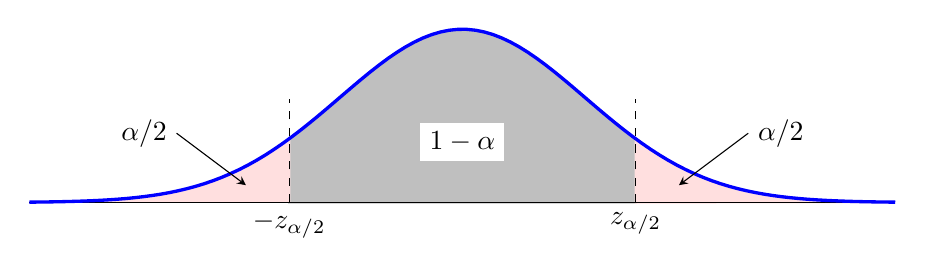
\begin{tikzpicture}[scale=2.2]
\draw[fill, color=gray!50!white, domain=-1:1, samples=100, thick]plot(\x, {exp(-\x*\x)})--(1,0)--(-1,0)--(-1,.368);
\draw[fill, color=pink!50!white, domain=-2.5:-1, samples=100, thick]plot(\x, {exp(-\x*\x)})--(-1,.368)--(-1,0);
\draw[fill, color=pink!50!white, domain=1:2.5, samples=100, thick]plot(\x, {exp(-\x*\x)})--(1,0)--(1,.368);

\node[fill=white] at (0,.35){$1-\alpha$}; 
\draw(-2.5,0)--(2.5,0);
\draw[domain=-2.5:2.5, samples=100, very thick, blue]plot(\x, {exp(-\x*\x)});
\draw[<-](-1.25,.1)--(-1.65,.4)node[left]{$\alpha/2$};
\draw[<-](1.25,.1)--(1.65,.4)node[right]{$\alpha/2$};
\draw[dashed](-1,0)node[below]{$-z_{\alpha/2}$}--(-1,.6);
\draw[dashed](1,0)node[below]{$z_{\alpha/2}$}--(1,.6);

\end{tikzpicture}
\end{center}
\end{frame}


\begin{frame}[fragile]{$z_{q}$的计算}
\begin{center}
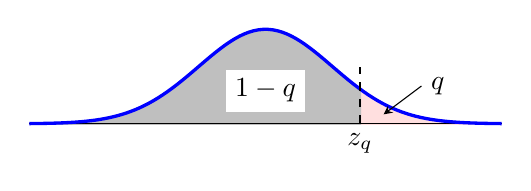
\begin{tikzpicture}[scale=1.2]
\draw[fill, color=pink!50!white, domain=1:2.5, samples=100, thick]plot(\x, {exp(-\x*\x)})--(1,0)--(1,.368);
\draw[fill, color=gray!50!white, domain=-2.5:1, samples=100, thick]plot(\x, {exp(-\x*\x)})--(1,0)--(-2.5,0);

\node[fill=white] at (0,.35){$1-q$}; 
\draw(-2.5,0)--(2.5,0);
\draw[domain=-2.5:2.5, samples=100, very thick, blue]plot(\x, {exp(-\x*\x)});
\draw[<-](1.25,.1)--(1.65,.4)node[right]{$q$};

\draw[dashed](1,0)node[below]{$z_{q}$}--(1,.6);
\end{tikzpicture}
\end{center}

Python的\verb|scipy|库中\verb|norm.isf|函数可以用于计算$z_q$值。\verb|isf|是Inverse Survival Function(反生存函数)的缩写。
\begin{lstlisting}
    from scipy import stats
    stats.norm.isf(q, loc, scale)
\end{lstlisting}
\begin{itemize}
    \item \verb|q| 正态分布上侧面积(概率)
    \item \verb|loc| 可选项,位置参数($\mu$),默认取值为0
    \item \verb|scale| 可选项,尺度参数($\sigma$),默认取值为1
\end{itemize}
\end{frame}


\begin{frame}[fragile]{标准差未知}
在实践中,往往是不知道样本标准差的。如果 样本量较小或总体标准差$\sigma$未知,此时可以利用样本标准差$s$来估计$\sigma$。
总体均值的区间以自由度为$(n-1)$的$t$分布为依据进行估计
\[t=\frac{\bar x-\mu}{s/\sqrt{n}}\sim t(n-1)\]

假设$\alpha$为置信度,总体均值近似($1-\alpha$)的可信度,分布在以下置信区间内:
\[\left[\bar x-t_{\alpha/2}(n-1)\frac{s}{\sqrt{n}},\; \bar x+t_{\alpha/2}(n-1)\frac{s}{\sqrt{n}}\right]\]
\end{frame}


\begin{frame}[fragile]{$t_q(n)$的计算}
Python的\verb|scipy|库中\verb|t.isf|函数可以用于计算$t_q(n)$值
\begin{lstlisting}
    from scipy import stats
    stats.norm.isf(q, n, loc, scale)
\end{lstlisting}
\begin{itemize}
    \item \verb|q| $t$分布上侧面积(概率)
    \item \verb|n| 自由度
    \item \verb|loc| 可选项,位置参数($\mu$),默认取值为0
    \item \verb|scale| 可选项,尺度参数($\sigma$),默认取值为1
\end{itemize}
\end{frame}

\section{金融数据时间序列分析}
\subsection{时间序列的含义}
\begin{frame}[fragile]{时间序列的含义}
最早的时间序列分析可以追
溯到7000年前的古埃及,
通过对尼罗河涨落的情况这
个时间序列的长期观察,掌
握了尼罗河泛滥的规律,古
埃及的农业迅速发展,从而
创建了古埃及灿烂的史前文
明

将尼罗河涨落的情况按
照时间的顺序把随机事
件的过程记录下来就构
成了一个时间序列

从科学的角度讲,按时
间顺序排列的一组随机
变量$X = \{x_1 , x_2,\ldots x_t\}$
称为时间序列(time series),其中的
$𝑥_n$称为时间序列的观测
值
\end{frame}


\begin{frame}[fragile]{时间序列的研究方法}
平稳时间序列:时间序列不存在趋势变化,其观察值围绕均值在某个固定的水平内上下波动
\begin{itemize}
    \item 时间序列的均值与时间变量无关
    \item 时间序列的方差与时间变量无关
    \item   时间序列的协方差只与时期间隔有关,与时间变量无关
\end{itemize}

\begin{block}{平稳时间序列分类}
   \begin{itemize}
    \item 纯随机序列:变化没有任何规律可循,不同时间点的观测
    值互不相关,不能从
    中找出规律进行模拟
    拟合,也无法由历史
    值推测未来值
    \item 非纯随机序列:平稳的非纯随机时间
    序列,则有很多模型
    可以用来拟合,其中
    最常用ARMA模型
\end{itemize} 
\end{block}

\end{frame}

\subsection{时间序列的检验}
\begin{frame}[fragile]{平稳性检验}
\begin{itemize}
    \item 图检验法:时序图、自相关图(基本判断)
    \item 统计检验法:构造检验统计量(辅助判断)
\end{itemize}

\end{frame}


\begin{frame}[fragile]{时序图检验}
    时间序列是平稳序列,则时序图
    中的观测值应围绕其均值,在一
    定范围内上下波动。反之,如果
    时序图有明显的趋势性或周期性,
    则该时间序列很可能不是平
    稳序列

时序图:以时间为横轴、以观测值为纵轴的时间序列折线图


\end{frame}


\begin{frame}[fragile]{时序图绘制}
\begin{lstlisting}
    df.plot(x=None, y=None, kind='line')
\end{lstlisting}
\begin{itemize}
    \item \verb|x|, \verb|y| 用来指定绘图的数据,对应\verb|df|中的{\color{red}列索引}
    \item \verb|kind| 设置绘图的类型,默认为折线图
\end{itemize}

\end{frame}

\begin{frame}[fragile]{举例:平安银行的数据}
\begin{lstlisting}
import pandas as pd
import matplotlib.pyplot as plt
data = pd.read_excel('平安银行.xlsx', index_col=0) 
data['收盘价'].plot() # 绘制股票收盘价的时间序列图
plt.xlabel('时间')
plt.ylabel('收盘价')  # 设置x轴、y轴的标签文本
plt.show()               # 图片显示
data['收益率'].plot()  # 绘制股票收益率的时间序列图
plt.xlabel('时间') 
plt.ylabel('收益率')  # 设置x轴、y轴的标签文本
plt.show()               # 图片显示
\end{lstlisting}


\end{frame}


\begin{frame}[fragile]{举例:平安银行的数据(cont.)}
以两个子图展示相关图片
\begin{lstlisting}
import pandas as pd;   import matplotlib.pyplot as plt
data = pd.read_excel('平安银行.xlsx', index_col=0) 
fig, axes = plt.subplots(nrows=1, ncols=2, figsize(14,6))
axes[0].plot(data['收盘价'])
axes[0].set_xlabel('时间'); axes[0].set_ylabel('收盘价')  
axes[1].plot(data['收益率'])  
axes[1].set_xlabel('时间'); axes[1].set_ylabel('收益率') 
plt.show()
\end{lstlisting}


\end{frame}

\begin{frame}[fragile]{自相关检验——自相关函数}
对于时间序列$X_t$,取样本$X_n=\{x_1,x_2,\ldots, x_n\}$,将$X_n$滞后$k$阶后形成的样本记为$X_{n+k}$,即:
\[X_{n+k}=\{x_{1+k},x_{2+k},\ldots, x_{n+k}\}\]
两者之间的协方差函数如下:
\[{\rm Cov}(X_n,X_{n+k})=\E\Big\{\big[X_n-\E(X_n)\big]\big[X_{n+k}-\E(X_{n+k})\big]\Big\}\]
两者之间的自相关函数(AutoCorrelation Function, ACF)如下:
\[\rho_k=\frac{{\rm Cov}(X_n,X_{n+k})}{\sigma_n \sigma_{n+k}},\qquad k=1,2,\ldots \]


\end{frame}

\begin{frame}[fragile]{自相关函数(cont.)}
    自相关函数可以度量同一事件在两个不同时期的相关程度。取值越大,意味着时间序列自身的记忆性越强,历史对当前的影响越大

    若时间序列是平稳的,则自相关函数只与间隔时间$k$有关,而与时间变量$n$无关,并且当$k$较大时,$X_n$与$X_{n+k}$应当相互独立,自相关系数为0

对于平稳时间序列而言,其自相关系数一般会快速减小至0附近,或者在某一阶后变为0(截尾);非平稳时间序列的自相关系数一般是缓慢下降(拖尾)。
\end{frame}


\begin{frame}[fragile]{自相关图的绘制}
\begin{lstlisting}
from statsmodels.graphics.tsaplots import plot_acf
plot_acf(x, ax=None, lags=None, alpha=0.05, 
            title='Autocorrelation')
\end{lstlisting}
\begin{itemize}
    \item \verb|x| 待检测的时间序列;
    \item \verb|ax| 绘制子图的选项,默认不绘制子图;
    \item \verb|lags| 可选项,表示滞后阶数的最大值,输入为整数值;
    \item \verb|alpha| 可选项,默认返回95\%的置信区间;
    \item \verb|title| 显示自相关图的标题
\end{itemize}
\end{frame}

\begin{frame}[fragile]{偏自相关图的绘制}
序列的偏自相关图(Partial AutoCorrelation Function, PACF),使用函数\verb|plot_pacf|绘制。用法与自相关图函数\verb|plot_acf|相同。偏自
相关图可用于时间序列ARMA模型定阶
\begin{lstlisting}
from statsmodels.graphics.tsaplots import plot_pacf
plot_pacf(x, ax=None, lags=None, alpha=0.05, 
            title='Partial Autocorrelation')
\end{lstlisting}
\end{frame}


\begin{frame}[fragile]{举例:平安银行收盘价和收益率的自相关与偏自相关图}
\normalsize
\begin{lstlisting}
from statsmodels.graphics.tsaplots import plot_acf, plot_pacf 
import matplotlib.pyplot as plt
fig, axes = plt.subplots(nrows=2, ncols=2, figsize=(10,10))
plot_acf(x, ax=axes[0,0], lags=30, title='ACF of close price') 
plot_pacf(x, ax=axes[0,1], lags=30, title='PACF of close price') 
plot_acf(y, ax=axes[1,0], lags=30, title='ACF of return') 
plot_pacf(y, ax=axes[1,1], lags=30, title='PACF of return') 
\end{lstlisting} 

绘制出的图,以$2\times 2$的子图排列,此处\verb|x|和\verb|y|分别对应平安银行收盘价和收益率序列
\end{frame}

\subsection{单位根检验}
\begin{frame}[fragile]{单位根的概念}
对于下列方程:
\[x_t=bx_{t-1}+a+\varepsilon\]
若$b=1$,则称为单位根。单位根的存在,意味着对应的序列$\{x_t\}$不平稳,无法对其进行预测

单位根检验法就是判断时间序列平稳性的方法之一,通常称作ADF检验(Augmented Dickey-Fuller test)
\end{frame}


\begin{frame}[fragile]{ADF检验}
原假设$H_0$是单位根存在,
序列不平稳;备择假设$H_1$是单位根不存
在,序列平稳
\begin{itemize}
    \item ADF的$T$-统计量的绝对值大于1\%,5\%,10\% 不同置信度水平下$T$-统计量的绝 对值,则拒绝原假设
    \item ADF的\verb|p-value|是指原假设为真的概率,如果\verb|p-value|值非常接近0,则拒绝原假设
\end{itemize}
\end{frame}


\begin{frame}[fragile]{平稳性检验}
python的\verb|statsmodels|库中,\verb|adfuller|函数可以用于单位根检验
\begin{lstlisting}
adfuller(x, regression='c', maxlag=None, store=False, regresults=False)
\end{lstlisting}
\begin{itemize}
    \item \verb|x| 待检验的时间序列; 
    \item \verb|regression| 回归方程中的参数设定,默认只包含常数项,可选参数有:\verb|ct|常数项和趋势项;\verb|ctt|常数项,线性二次项;\verb|nc|没有常数项和趋势项
    \item \verb|maxlag| 最大延迟期数,需输入整数值; 
    \item \verb|store| 默认不返回adf统计信息的结果; 
    \item \verb|regresults|  默认返回完整的回归结果
\end{itemize}
\end{frame}


\begin{frame}[fragile]{平稳性检验举例}
\begin{lstlisting}
from statsmodels.tsa.stattools import adfuller
dftest1 = adfuller(data['收盘价']); print(dftest1)
dftest2 = adfuller(data['收益率']); print(dftest2)
\end{lstlisting}

\begin{block}{结果解读}
输出结果以元组形式展现:第一个值表示$T$统计量;
第二个值是 \verb|p-value|,即$p$值,表示$T$统计量对应的概率;第三个值是滞后阶数;第四个值是观测值数量;第五个是字典,存储的是1\%、5\%、10\%三个水平下的$T$统计量取值
\end{block}
\end{frame}

\subsection{纯随机性检验}
\begin{frame}[fragile]{纯随机序列}
    纯随机序列也称为白噪声(white noise),序列中任意两个不同时间的数据相互独立、互不相关,数据间没有规律可循,
    不具有建模分析的价值

    纯随机性检验的目的就是剔除掉纯随机序列,检测那些序列值之间具有密切相关关系,历史数据对未来的发展具有一定影响的非纯随机序列
\end{frame}


\begin{frame}[fragile]{纯随机性检验}
\begin{block}{Barlett定理}
如果一个时间序列是纯随机的,得到一个观察期数为$n$的序列$x_t$, 那么该序列的滞后$k\; (k=\ne 0)$期的样本自相关系数$\hat\rho_k$将近似服从均值为零、 方差为$1/n$的正态分布
\[\hat\rho_k \sim \mathcal{N}\left(0,\frac{1}{n}\right),\qquad \forall k\ne 0 \]
\end{block}

根据Barlett定理,可以通过构造$Q$统计量和$LB$(Ljung-Box)统计量来检验序列的纯随机性
\end{frame}


\begin{frame}[fragile]{纯随机性检验——$Q$统计量}
Box 和Pierce推导出$Q$统计量
\[Q=n\sum^m_{k=1}\hat \rho^2_k \mathop{\sim}^{\rm asy.}  \chi^2(m)\]
其中:$n$为序列观测期数;$m$为设定的滞后阶数

\begin{block}{说明:}
    $Q$统计量适用于$n$取值很大(大样本)的场合,此处只是渐近地(asymptotic)服从自由度为$m$的$\chi^2$分布
\end{block}
\end{frame}


\begin{frame}[fragile]{纯随机性检验——$LB$统计量}
在实际应用中,人们发现$Q$统计量在大样本场合(观测期 数$n$ 很大的场合)检验效果 很好, 但在小样本场合不太精确。为了弥补这一缺陷, 又推导出了$LB$(Ljung-Box)
统计量
\[LB=n(n+2) \sum^m_{k=1}\frac{\hat \rho^2_k }{n-k} \mathop{\sim}^{\rm asy.} \chi^2(m)\]
\begin{block}{说明:}
    实际上 $LB$ 统计量就是$Q$统计量的修正,所以人们 习惯把它们统称为 $Q$ 统计量,分别记作$Q_{BP}$和$Q_{LB}$统计量
\end{block}
\end{frame}


\begin{frame}[fragile]{统计量的检验}
\begin{itemize}
    \item 原假设$H_0$:滞后期$\le m$的序列值之间相互独立
    \item 备择假设$H_1$:滞后期$\le m$的序列值之间有相关性
\end{itemize}

python中的\verb|statsmodels|模块中的\verb|acorr_ljungbox|函数可用于$Q$统计量和$LB$统计量计算
\begin{lstlisting}
from statsmodels.stats.diagnostic import acorr_ljungbox
acorr_ljungbox(x, lags=None, boxpierce=False)
\end{lstlisting}
\begin{itemize}
    \item \verb|x| 待检验的随机序列;
    \item \verb|lag| 滞后阶数,一般为整数值;
    \item \verb|boxpierce| 默认不返回 $Q$统计量的结果
\end{itemize}

\end{frame}


\begin{frame}[fragile]{统计量的检验结果解读}
\begin{lstlisting}
from statsmodels.stats.diagnostic import acorr_ljungbox
Q_test = acorr_ljungbox(x, lags=None, boxpierce=True)
print(Q_test)
\end{lstlisting}
输出结果以元组形式展现:第一个值表示$LB$统计量的取值,第二个值是对应的$p$值;若\verb|boxpierce=True|,则元组会有四个元素,前两个值的含义同上,第三个值是$Q$统计量取值,第四个是对应的$p$值
\end{frame}

\section{时间序列建模}
\subsection{平稳化处理}
\begin{frame}[fragile]{平稳化处理}
对于具有趋势的非平稳时间序列来说,差分(difference)是去除非平稳性的最便捷工具

差分就是序列中相邻两个数之间的变化量。记序列为$X_n=\{x_1,x_2,\ldots,x_n\}$,则:
\[\Delta x_t=x_t-x_{t-1}\]

\begin{center}
\begin{tikzpicture}
\node [fill=cyan!60!white, circle] (A) at (0,0) {$X_n$};
\node [fill=cyan!40!white,circle ] (B) at (3,0) {$\Delta x$};
\node [fill=cyan!20!white,circle ] (C) at (6,0) {$\Delta_2 x$};
\node  (D) at (8,0) {$\cdots$};
\draw[->, color=magenta, thick](A)--node[above]{一阶差分}(B);
\draw[->, color=magenta, thick](B)--node[above]{一阶差分}(C);
\draw[->, color=magenta, thick](C)--(D);

\end{tikzpicture}
\end{center}

\end{frame}


\begin{frame}[fragile]{时间序列的差分}
Python的Pandas库中,\verb|.diff|方法可用来进行时间序列的差分
\begin{lstlisting}
    df.diff(periods=1, axis=0)
\end{lstlisting}
\begin{itemize}
    \item \verb|df|为Dataframe 或者Series类型的数据
    \item \verb|periods| 差分的阶数,输入值为整数值,默认值为1
    \item \verb|axis| 移动的方向,默认按列差分;选择\verb|1/'columns'| 按行差分
\end{itemize}

\begin{block}{说明:}
    差分后,因序列首个数值缺乏差分对象,会导致差分后的序列首位数值缺失,可用\verb|dropna|函数进行删除
\end{block}
\end{frame}

\begin{frame}[fragile]{举例:对平安银行收盘价的差分序列进行平稳性检验}
\begin{lstlisting}
import pandas as pd
import numpy as np
from statsmodels.tsa.stattools import adfuller
# data为平安银行数据,其中包含收盘价和收益率两列数据
# 对收盘价进行一阶差分,并去掉缺失值
data_diff1 = data['收盘价'].diff(1).dropna() 
dftest = adfuller(data_diff1) # 平稳性检验
print(dftest)
\end{lstlisting}
\end{frame}


\subsection{ARMA模型}
\begin{frame}[fragile]{ARMA模型}
ARMA模型(AutoRegression Moving Average)全
称是自回归移动平均模型,是目前最常用的拟合平稳时
间序列的模型

\begin{block}{${\rm ARMA}(p,q)$模型的形式}
    \[\begin{split}
 x_t&= \varphi_0+\varphi_1x_{t-1}+\cdots +\varphi_p x_{t-p}+\varepsilon_t-\theta_1\varepsilon_{t-1}-\cdots -\theta_q\varepsilon_{t-q}         \\
&=\varphi_0 + \sum_{m=1}^{p}\varphi_m x_{t-m}+\varepsilon_t-\sum_{n=1}^{q}\theta_n\varepsilon_{t-n} 
    \end{split} \]
\end{block}

${\rm ARMA}(p,q)$模型有两个特例,分别是AR$(p)$模型和MA$(q)$模型

\end{frame}


\begin{frame}[fragile]{AR模型}
    AR模型又称为自回归模型(AutoRegression model),是ARMA模型中序列$x_t$只受历史观测值影响,而不受历史随机扰动因素影响的特例,即 ${\rm ARMA}(p,q)$模型中$q=0$时的情况
    \[\begin{split}
x_t&= \varphi_0+\varphi_1x_{t-1}+\cdots +\varphi_p x_{t-p}+\varepsilon_t   \\
&=\varphi_0 + \sum_{m=1}^{p}\varphi_m x_{t-m}+\varepsilon_t
    \end{split} \]
其中:$\varphi_p\ne 0$,$\varepsilon_t$是随机白噪声序列,且与$t$时刻之前的序列值无关
\end{frame}

\begin{frame}[fragile]{MA模型}
    MA模型又称为移动平均模型(Moving Average model),是ARMA模型中序列$x_t$的取值在均值附近,只受历史观测值随机扰动因素的影响,而与历史观测值无关的特例,即 ${\rm ARMA}(p,q)$模型中$p=0$时的情况
    \[\begin{split}
 x_t&= \mu+\varepsilon_t-\theta_1\varepsilon_{t-1}-\cdots -\theta_q\varepsilon_{t-q}         \\
&=\mu+\varepsilon_t-\sum_{n=1}^{q}\theta_n\varepsilon_{t-n} 
    \end{split} \]
其中:$\theta_q\ne 0$,$\varepsilon_t$是随机白噪声序列

\begin{block}{说明:}
    在实际应用中,用${\rm ARMA}(p,q)$模型
拟合实际数据时,$p$
和$q$的数值很少超过2
\end{block}
\end{frame}


    \subsection{时间序列建模}
\begin{frame}[fragile]{非随机时间序列的建模过程}
\begin{enumerate}
    \item 将时间序列从某一时刻截断分成历史数据(训练集);“未来”数据(测试集)
    \item 模型定阶:用训练集数据确定差分阶数$d$和ARMA模型中的$p$、$q$值
    \item 拟合ARMA模型:使用$p$、$q$、$d$值,拟合ARMA模型
    \item 预测并检验:用模型进行预测,并
    计算预测值和测试集中真实值的残
    差平方和,检验模型的效果
\end{enumerate}
\end{frame}

\begin{frame}[fragile]{模型定阶}
    对训练集数据进行平稳性检验,
    如果不平稳,则差分至平稳,
    平稳的差分阶数即为$d$

    绘制训练集数据的自相关图(ACF)和偏
    自相关图(PACF)。图中悬垂线快速衰减
    到0或阴影区域时,前者的横坐
    标为$q$,后者的横坐标为$p$

    python \verb|pmdarima|库中,\verb|auto.arima|函数可以自动尝试不同的阶数组合并挑选出可能的最优模型,从而自
    动定阶

\begin{block}{注意:}
    \verb|pmdarima|库不包含在Anaconda等Python开发平台中,需要单独安装,联网安装命令为:
\begin{lstlisting}
    pip install pmdarima
\end{lstlisting}
\end{block}
\end{frame}


\begin{frame}[fragile]{模型定阶(cont.)}
\begin{lstlisting}
import pmdarima as pm
pm.auto_arima(x, d=None, max_p=3, max_q=3, start_p=0, start_q=0, information_criterion='aic', test='adf', m=1, seasonal=True, trace=True)
\end{lstlisting}
\begin{itemize}
    \item \verb|x| 需要拟合的数据序列
    \item \verb|d| 指定差分阶数,默认自动计算差分阶数
    \item \verb|start_p|, \verb|max_p| 指定AR模型的阶数范围
    \item \verb|start_q|, \verb|max_q| 指定MA模型的阶数范围
    \item \verb|information_criterion| 指定最优模型评判标
    准(信息准则),默认是赤池信息准则
\end{itemize}


\end{frame}

\begin{frame}[fragile]{模型定阶(cont.)}
\begin{lstlisting}
import pmdarima as pm
pm.auto_arima(x, d=None, max_p=3, max_q=3, start_p=0, start_q=0, information_criterion='aic', test='adf', m=1, seasonal=True, trace=False)
\end{lstlisting}
\begin{itemize}
    \item \verb|test| 默认使用ADF检验差分的阶数\verb|d|
    \item \verb|m| 季节性周期长度,默认不考虑周期性。\verb|m=4|表示季度数据;\verb|m=12|表示月度数据
    \item \verb|seasonal| 默认考虑季节性,当\verb|m=1|时,\verb|seasonal=False|
    \item \verb|trace| 默认不报告尝试过的ARIMA模型结果
\end{itemize}


\end{frame}

\begin{frame}[fragile]{举例:平安银行收盘价数据的模型定阶}
\begin{lstlisting}
from pmdarima import auto_arima
model = auto_arima(data['收盘价'], start_p=0, start_q=0, 
        information_criterion='aic', test='adf', max_p=3, 
        max_q=3, m=1, d=None, seasonal=False, trace=True) 
print(model)      # 显示最佳拟合模型
\end{lstlisting}

\begin{block}{说明:}
输出结果当中报告了拟合过程中考虑到的各种ARIMA模型,并且通过AIC指标直接获取了最优的拟合模型
\end{block}
\end{frame}

\begin{frame}[fragile]{模型拟合}
模型定阶后,确定了$p,q,d$的值,将参数和序列历史数据代入ARIMA模型,就可对时间序列进行拟合

\begin{center}
    \begin{tikzpicture}
\node[fill=cyan!40!white] (A) at (0,0) {建立一个空白的ARIMA对象};
\node[fill=green!40!white] (A1) at (0,-1.5) {将参数和历史数据代入对象};
\node[fill=magenta!40!white] (A2) at (0,-3) {通过\texttt{fit}方法对模
型拟合激活};
\draw[->, thick, color=blue](A)--(A1);
\draw[->, thick, color=blue](A1)--(A2);
    \end{tikzpicture}
\end{center}
\end{frame}


\begin{frame}[fragile]{模型对象的建立及拟合}
Python的\verb|statsmodels|库中,\verb|ARIMA|函数可以用于建立模型对象
\begin{lstlisting}
from statsmodels.tsa.arima.model import ARIMA
model = ARIMA(endog, order=(p, d, q))
\end{lstlisting}
\begin{itemize}
    \item \verb|endog| 可选项,观察到的时间序列过程
    \item \verb|order| ARMIA模型的阶数,默认值为\verb|(0, 0, 0)|
\end{itemize}

Python中用于模型拟合的函数为\verb|fit|
\begin{lstlisting}
    results = model.fit()
\end{lstlisting}
\end{frame}


\begin{frame}[fragile]{模型对象的结果输出}
\begin{lstlisting}
results = model.fit()
print(results.summary()) # 输出模型的拟合结果及对应的各统计量
pred = results.predict()
print(pred)         # 输出根据设定的模型产生的预测数据序列
print('RSS: %.4f' %sum((pred- data['收盘价'])**2))  
# 输出模型的残差平方和(RSS)
\end{lstlisting}
\end{frame}


\section{投资组合相关性分析}
\subsection{投资组合理论}
\begin{frame}[fragile]{投资组合理论概述}
 投资组合是现代金融学界的核
心课题之一,投资组合的核心
问题是:投资者如何将合理分
配证券资产,以实现在既定风
险下收益最大化

马科维茨(H. Markowitz)用证券的期望收益率
来衡量投资的期望收益水平,
用收益率的方差来衡量投资的
风险。在投资者值关注“期望
收益率”和“方差”的前提下,
推导出结论:投资者应该通过
同时购买多种证券而不是一种
证券进行分散化投资。因此投
资组合理论通常也称为分散投
资理论,简单来说就是“不把
所有的鸡蛋放进同一篮子里”
\end{frame}


\begin{frame}[fragile]{马科维茨投资组合理论基本假设}
\begin{itemize}
    \item 投资者是风险规避的,追求期望效用最大化;
    \item 投资者根据收益率的期望值与方差来选择投资组
    合;
    \item 所有投资者处于同一单期投资期。
\end{itemize}

在满足以上假设的条件下,以资产权重$w_i$为变量,在
期望收益限制条件下,求解使得投资组合风险${\rm Var}(r_p)$最小
时的最优投资比例,其优化模型的数学公式为:
\[\begin{split}
    \min{\rm Var}(r_p)&=\sum^n_{i=1}\sum^n_{j=1} w_iw_j {\rm Cov}(r_i,r_j)\\
    {\rm s.t.}\qquad \E(r_p)&=\sum^n_{i=1} w_ir_i,\quad \sum^n_{i=1} w_i=1
\end{split} \]

\end{frame}



\begin{frame}[fragile]{投资组合理论(cont.)}
    投资组合在实际优化过程中会存在很
    多中资金分配方案,需要选择风险
    (方差)最小的方案。然后在不同期
    望收益水平下,得到相应的使方差最
    小的资产分配方案,这些解构成了最
    小方差组合(有效组合)
    
    有效组合
    的收益期望和相应的最小方差形成的
    曲线,就是有效组合投资的前沿
    (efficient frontier)
\end{frame}


\subsection{皮尔逊相关系数}
\begin{frame}[fragile]{皮尔逊相关系数的概念}
皮尔逊相关系数(Pearson
    correlation coefficient)用于度
    量两个变量之间的{\color{red}线性相关性}的
    指标
\[\rho_{X,Y}=\frac{{\rm Cov}(X,Y)}{\sigma_X\sigma_Y}=\frac{\E[(X-\mu_X)(Y-\mu_Y)]}{\sigma_X\sigma_Y} \]
    两个序列之间的相关系数是其协方差
    和标准差的商,其取值范围为$[−1,1]$

\begin{block}{说明:}
\begin{itemize}
    \item $\rho_{X,Y}=1$,存在确切的线性正相关;
    \item $\rho_{X,Y}=0$,不存在任何线性相关性;
    \item  $\rho_{X,Y}=-1$,存在确切的线性负相关。
\end{itemize}
\end{block}
\end{frame}


\begin{frame}[fragile]{皮尔逊相关系数的计算}
    Python的Pandas库,可计算列的成对相关性并生成矩阵
\begin{lstlisting}
    df.corr(method='pearson', min_periods=1)
\end{lstlisting}
\begin{itemize}
    \item \verb|method| 选择使用哪种相关分析方法,默认是使用皮尔逊相关系数,还可以设置为\verb|'kendall'|或\verb|'spearman'|
    \item \verb|min_periods| 代表每个“列对”指定所需的最小非NA观测数,以便
    获得有效结果
\end{itemize}

\begin{block}{说明:}
    该函数会自动从计算中排除\verb|NA|和\verb|null|
\end{block}
\end{frame}

\begin{frame}[fragile]{相关系数的可视化}
    常用seaborn库中的\verb|heatmap|函数,来绘制热图(heat map)以便于观察相关矩阵
\begin{lstlisting}
from seaborn import heatmap
heatmap(data, cmap=None, annot=False, linewidths=0, annot_kws=None)
\end{lstlisting}
\begin{itemize}
    \item \verb|data| 要显示的数据
    \item \verb|cmap| 选填项,\verb|matplotlib|的colormap名称或颜色对象
    \item \verb|annot| 选填项,默认不在热图的每个方格中写入数据
    \item \verb|linewidths| 热图矩阵之间的间隔大小,默认为0
    \item \verb|annot_kws| 热图上每个方格数据字体的大小
\end{itemize}

\end{frame}



\begin{frame}[fragile]{协方差矩阵的计算}
    相关系数只反应了证券之间的线性关系,
    即股票之间每次涨跌时的类似程度,但
    并不能告诉股票之间的波动(变化幅度)
    情况,而协方差矩阵则包含这一信息

    当协方差为正数时,代表股票都同方向
    偏离各自均值,可帮助了解到股票此时变
    动幅度距离其平均幅度有多大

    Python的Pandas库,可计算列的成对协方差并生成协方差矩阵
\begin{lstlisting}
    df.cov(min_periods=None)
\end{lstlisting}
\end{frame}


\begin{frame}[fragile]{相关系数的显著性检验}
    皮尔逊相关系数可以量化两只股票间的相关关系
    大小,但需要进一步考虑这种相关关系是否在统
    计上显著
\begin{itemize}
    \item 原假设:两只序列的线性相关关系不显著;
    \item 备择假设:两只序列的线性相关关系显著。
\end{itemize}
如果计算出的$p$-value值接近于零,表明接受假
设的概率不大,则拒绝原假设,认为两只序列的
线性相关关系显著。
\end{frame}


\begin{frame}[fragile]{举例:协方差矩阵的计算}
以15支股票的日收益率数据为例,计算协方差矩阵并画出热图
\begin{lstlisting}
import pandas as pd
cov_mat = stockreturns.cov()
print(round(cov_mat, 5))  # 保留五位小数,也可以写成以下形式:
print(cov_mat.round(5))
# 画热图
import matplotlib.pyplot as plt
from seaborn import heatmap
heatmap(cov_mat.round(3), cmap='rainbow', linewidth=2, 
        annot=True)
\end{lstlisting}
\end{frame}


\begin{frame}[fragile]{相关系数的显著性检验(cont.)}
在Python的scipy库中,\verb|pearsonr|函数可以计算相关系数,并获得双边检验的$p$值
\begin{lstlisting}
from scipy.stats import pearsonr
pearsonr(x, y)
\end{lstlisting}

输出的结果是一个元组,第一个值表示皮尔逊相关系数,第二个值是对应的$p$值
\end{frame}


\subsection{等权重投资组合}
\begin{frame}[fragile]{等权重投资组合}
    最容易理解的投资策略:
\begin{itemize}
    \item 投资方案里资金将均分到每支证券里;
    \item 所有证券的权重都相等
    \[w_1=w_2=\cdots=w_n=\frac{1}{n}\]
\end{itemize}    

构造一个等权的权重序列,需要在numpy库中使用\verb|repeat|函数
\begin{lstlisting}
    numpy.repeat(a, repeats, axis=None)
\end{lstlisting}
\begin{itemize}
    \item \verb|a| 输入需要重复的元素或数组
    \item \verb|repeats| 每个元素的重复次数
\end{itemize}
\end{frame}


\begin{frame}[fragile]{等权重投资组合权重序列的构造}
    让15支股票的每支组合权重为1/15,构造权重序列
\begin{lstlisting}
import numpy as np
numstocks = 15  
portfolio_weights = np.repeat(1/numstocks, numstocks) 
\end{lstlisting}
\end{frame}


\begin{frame}[fragile]{构造等权证券组合}
\begin{lstlisting}
# 在15支股票收益率矩阵中,按列依次乘以权重系数 
WeightedReturns = stockreturns.mul(portfolio_weights, axis=1) 
# 将加权后的15支股票收益率进行相加,构造投资组合序列
portfolio_ew = WeightedReturns.sum(axis=1) 
print(portfolio_ew)
\end{lstlisting}
\begin{center}
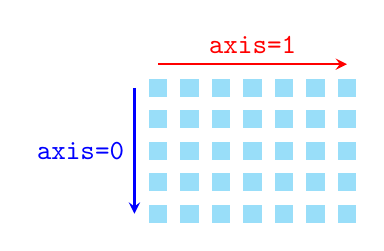
\begin{tikzpicture}[scale=.4]
\foreach \x in {1,2,...,7}
   \foreach \y in {1,2,...,5}
    \node[fill=cyan!40!white] at (\x,\y){\quad};
\draw[->,thick, red](1,5.75)--node[above]{\texttt{axis=1}}(7,5.75);
\draw[->,thick, blue](.25,5)--node[left]{\texttt{axis=0}}(.25,1);
\end{tikzpicture}
\end{center}
\end{frame}


\begin{frame}[fragile]{证券组合的特征}
只看日收益率,很难观察到投资组合的长期收益,要 知道投资中上期未的本利和是作为下一期的本金,也 就是通俗上说的“利滚利”。

客户实际上获取的收益率是累乘收益率
\[\begin{split}
    return &= (1+r_1)(1+r_2)\cdots(1+r_n)-1\\
&=\prod^{n}_{i=1}(1+r_i) -1
\end{split} \]

\end{frame}




\begin{frame}[fragile]{累乘}
    Python中\verb|cumprod|函数可以实现收益率的累乘({\color{red}cum}ulative {\color{red}prod}uct)计算

\begin{lstlisting}
    df.cumprod(axis=0, skipna=True)
\end{lstlisting}

\begin{itemize}
    \item \verb|axis| 默认按行计算, \verb|axis=1|代表对列计算
    \item \verb|skipna| 默认计算时自动忽略\verb|NA|和\verb|null|
\end{itemize}
返回累乘构成的Series或DataFrame

\end{frame}



\begin{frame}[fragile]{对投资组合的日收益率计算累乘收益率并绘图}
\begin{lstlisting}
import pandas as pd
import matplotlib.pyplot as plt
plt.figure(figsize=(6,5), dpi=100)      # 设置画布尺寸及清晰度
Cum_Returns=((1+portfolio_ew).cumprod()-1) 
Cum_Returns.plot(label='equally-weighted portfolio')  
#  或者写成以下形式:
plt.plot(Cum_Returns, label='equally-weighted portfolio')
plt.legend() # 添加图例,文字来自于plot中的label
plt.show()
\end{lstlisting}
\end{frame}


\end{document}